\chapter{Questionnaire}
\label{ch:questionnaire_appendix}
The questionnaire presented below was answered by 9 respondents with strong interest in football betting. 

\section{Questions}
This questionnaire intends to collect information about the way football punters make their betting decisions (decide which team to bet on).

The questionnaire should only take around five minutes to fill in and your answers will be used to aid the development of a web application simulating the football betting experience. The future application will provide its users with all the necessary football statistics (without going too much into detail) and allow them to participate in the prediction process by making their own prediction formula. 

\textbf{Question 1}\par
\textbf{How many times a week do you bet on football or other sporting events?}
\begin{itemize}
	\item Less than once a week
	\item 1 time a week
	\item 2-3 times a week
 	\item More than 3 times a week
 \end{itemize}
 
\textbf{Question 2}\par
\textbf{How many sources of information (websites, newspapers, your favourite mobile app) do you look into before making your placing your bet?}\par
\emph{For example, if you use 2 different websites (such as BBC News and Whoscored.com), the answer is 2.}
 \begin{itemize}
 	\item None
 	\item 2-3 sources
 	\item More than 3 sources
 \end{itemize}
 
\textbf{Question 3}\par
\textbf{Please specify the sources of information that you use to support your decision.}
 \begin{itemize}
	 \item TV programmes
	 \item Sports info websites (e.g., BBC News, The Guardian)
	 \item Football info websites (e.g., whoscored.com, squawka.com)
	 \item Gambling websites (e.g., Bet365, Ladbrokes)
	 \item Betting communities or forums (e.g.,OLGB.com)
	 \item Social Networks (e.g., betting tips from football experts on Twitter)
	 \item Printed media (newspapers)
	 \item Friend's advice
	 \item Mobile apps
	 \item Specify your own: 
\end{itemize}
  
\textbf{Question 4}\par
\textbf{What main factors do you take into account before placing a bet?}\par
\emph{Choose more than one or add your own}
 \begin{itemize}
	 \item Form
	 \item League position
	 \item Result of the previous match for each team
	 \item Home/Away performance so far in the season
     \item Change of a team manager
     \item Injuries/suspensions of players
	 \item Weather
	 \item Own hunch
	 \item Specify your own: 
\end{itemize}
 
\textbf{Question 5}\par
\textbf{Do you record your betting performance?}
\begin{itemize} 
 \item Yes
 \item No
\end{itemize}

\textbf{Question 6}\par
\textbf{What statement describes you best?}
 \begin{itemize}
 	\item I only use one bookmaker to place my bets
	\item I compare the odds several bookmakers and choose the best bookmaker for each match
\end{itemize}
 
\textbf{Question 7}\par
\textbf{Would you find a web application allowing you to participate in the prediction of a match result by making up you own prediction formula useful?}
\begin{itemize}
	\item Yes
	\item No
	\item Not sure
 \end{itemize}
 
\section{Answers}

\noindent
\begin{sidewaystable}
\begin{tabular}{
  |p{\dimexpr.1\linewidth-2\tabcolsep-1.3333\arrayrulewidth}% column 1
  |p{\dimexpr.2\linewidth-2\tabcolsep-1.3333\arrayrulewidth}% column 2
  |p{\dimexpr.2\linewidth-2\tabcolsep-1.3333\arrayrulewidth}% column 3
  |p{\dimexpr.5\linewidth-2\tabcolsep-1.3333\arrayrulewidth}|% column 4
  }
  \hline
  \centering Respondent  & \centering Question 1  & \centering Question 2 & \centering\arraybackslash Question 3   \\ \hline
  1 & 1 time a week & 2-3 sources & Sports info websites (e.g., BBC News, The Guardian), Football info websites (e.g., whoscored.com, squawka.com) \\ \hline
  2 & Less than once a week & 2-3 sources & TV programmes, Printed media (newspapers) \\ \hline
  3 & 2-3 times a week & 2-3 sources & TV programmes, Printed media (newspapers), Friends advice \\ \hline
  4 & More than 3 times a week & More than 3 sources & TV programmes, Sports info websites (e.g., BBC News, The Guardian), Gambling websites (e.g., Bet365, Ladbrokes), Betting communities or forums (e.g.,OLGB.com), Social Networks (e.g., betting tips from football experts on Twitter), Mobile apps \\ \hline
  5 & More than 3 times a week & 2-3 sources & TV programmes, Gambling websites (e.g., Bet365, Ladbrokes), Printed media (newspapers) \\ \hline
  6 & Less than once a week & 2-3 sources & Football info websites (e.g., whoscored.com, squawka.com) \\ \hline
  7 & More than 3 times a week & 2-3 sources & Football info websites (e.g., whoscored.com, squawka.com), Gambling websites (e.g., Bet365, Ladbrokes), Mobile apps \\ \hline
  8 & Less than once a week & 2-3 sources & TV programmes, Sports info websites (e.g., BBC News, The Guardian), Printed media (newspapers) \\ \hline
  9 & 2-3 times a week & 2-3 sources & Sports info websites (e.g., BBC News, The Guardian) \\ \hline
\end{tabular}
\\[10pt]
\caption{Table illustrating answers to questions 1-3 in the target audience questionnaire}
\end{sidewaystable}

\noindent
\begin{sidewaystable}
\begin{tabular}{
  |p{\dimexpr.1\linewidth-2\tabcolsep-1.3333\arrayrulewidth}% column 1
  |p{\dimexpr.3\linewidth-2\tabcolsep-1.3333\arrayrulewidth}% column 2
  |p{\dimexpr.1\linewidth-2\tabcolsep-1.3333\arrayrulewidth}% column 3
  |p{\dimexpr.4\linewidth-2\tabcolsep-1.3333\arrayrulewidth}% column 4
  |p{\dimexpr.1\linewidth-2\tabcolsep-1.3333\arrayrulewidth}|% column 5
  }
  \hline
  \centering Respondent  & \centering Question 4  & \centering Question 5 &  \centering Question 6 & \centering\arraybackslash Question 7   \\ \hline
  1  & Form, League position, Result of the previous match for each team, Own hunch & No & I only one bookmaker to place my bets & Yes \\ \hline
  2 & Form, League position, Injuries/suspensions of players & No & I only use one bookmaker to place my bets & Not sure \\ \hline
  3 & Form, League position, Home/Away performance so far in the season, Own hunch & No & I compare the odds several bookmakers and choose the best bookmaker for each match & Yes \\ \hline
  4  & Form, League position, Result of the previous match for each team, Home/Away performance so far in the season, Own hunch & No & I only use one bookmaker to place my bets & Yes \\ \hline
   5 & Form, League position, Home/Away performance so far in the season, Change of a team manager & No & I compare the odds several bookmakers and choose the best bookmaker for each match & Yes \\ \hline
   6 & Form, Own hunch & No & I only use one bookmaker to place my bets & No \\ \hline
   7 & Form, Home/Away performance so far in the season, Injuries/suspensions of players & No & I only use one bookmaker to place my bets & Yes \\ \hline 
   8 & Form, League position, Result of the previous match for each team, Injuries/suspensions of players, Own hunch & No & I only use one bookmaker to place my bets & Yes \\ \hline
   9 & Form, Own hunch, Whether or not the odds appear to offer good value & No & I only use one bookmaker to place my bets & Yes \\ \hline
  \end{tabular}
 \caption{Table illustrating answers to questions 4-7 in the target audience questionnaire}

\end{sidewaystable}

\chapter{Wireframes}
\label{ch:wireframes}
When the app is launched it silently registers with the server
allowing the user to use the app immediately. The user is then shown
the middle-top screen.
\begin{enumerate}
\item From the middle top screen, the user can follow arrow 1 by
  clicking on the middle button "Pick Mission'' to pick a Mission
  (Run around Arran or Egg for example) and then pick a start and
  end location. After confirming these choices, the user is taken
  back to the middle top screen, or at any time can click the
  "Home'' button to return. 
\item The user can also view their current acheivements by clicking
  the "Achievements" button on the middle top screen, following
  arrow 2. These achievements will be grouped by tabs by category -
  Distance, Time, Stage and Mission based achievements.
\item The user can follow arrow 3 from the middle top screen to
  notify the app that they are starting an exercise period, telling
  the app to track their distance. If a Mission and start and end
  location are not picked (as in point 1) then they will instead be
  redirected to this screen and are unable to start exercising until
  this choice has been made. Once they have successfully advanced to
  this screen, it will display their current progress as they move
  showing the user how close to completion of their current stage
  and overall route they are. 
\item When the user has finished exercising, they will click the
  "End Session'' button and be taken to the first summary screen -
  following arrow 4. Here statistics from their exercise will be
  shown and the option to share this on several social media
  outlets.
\item The user can then move to the second and final summary screen,
  following arrow 5, where they will be shown any achievements they
  were awarded during that session. The user will also have the
  option to share these on social media outlets. From here, the user
  can click the "Home" button and be taken back to the middle top
  screen. 
\end{enumerate}
\begin{figure}[H]
  \centering
  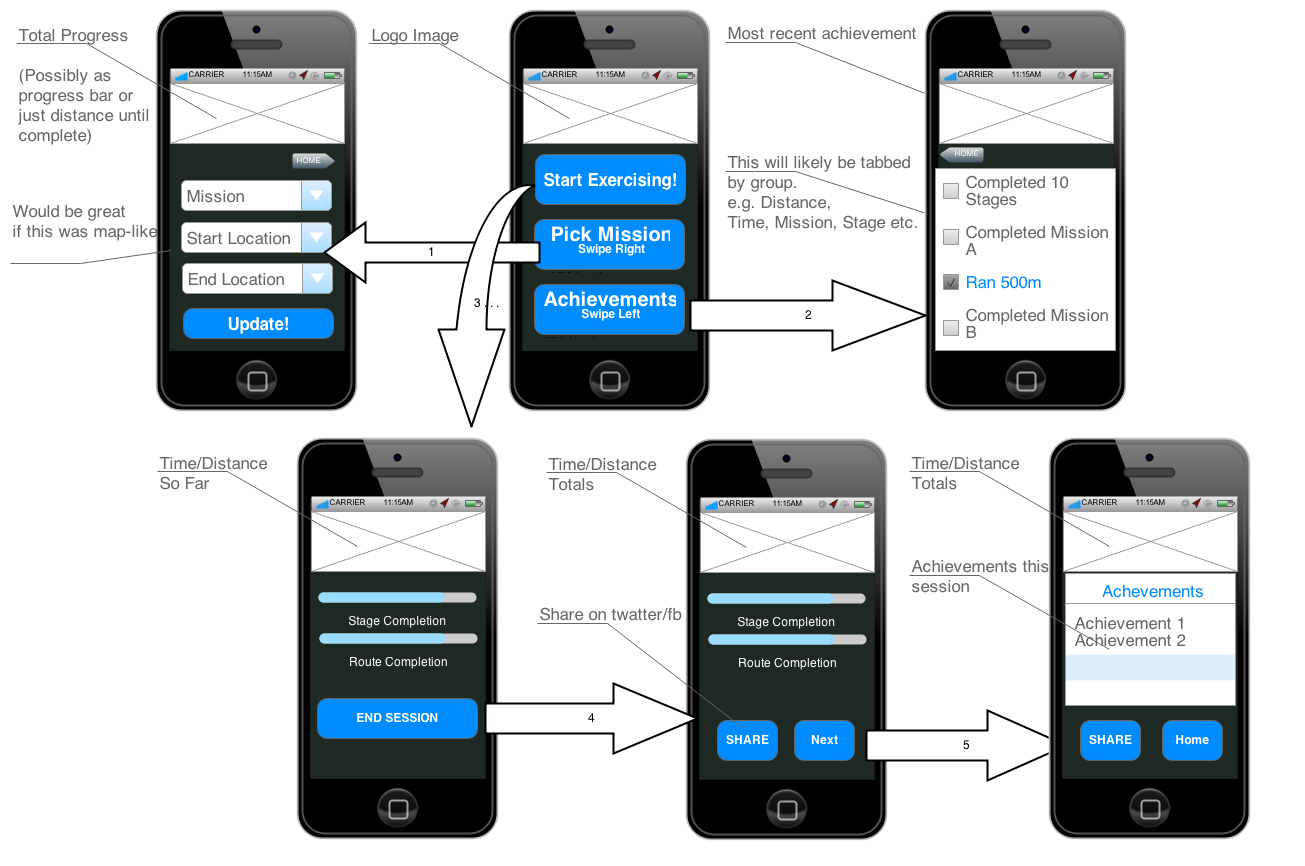
\includegraphics[width=\linewidth]{appendix/images/wireframes.png}
  \caption{Wireframes, initial design}
  \label{wireframes_1}
\end{figure}
\begin{figure}[H]
  \centering
  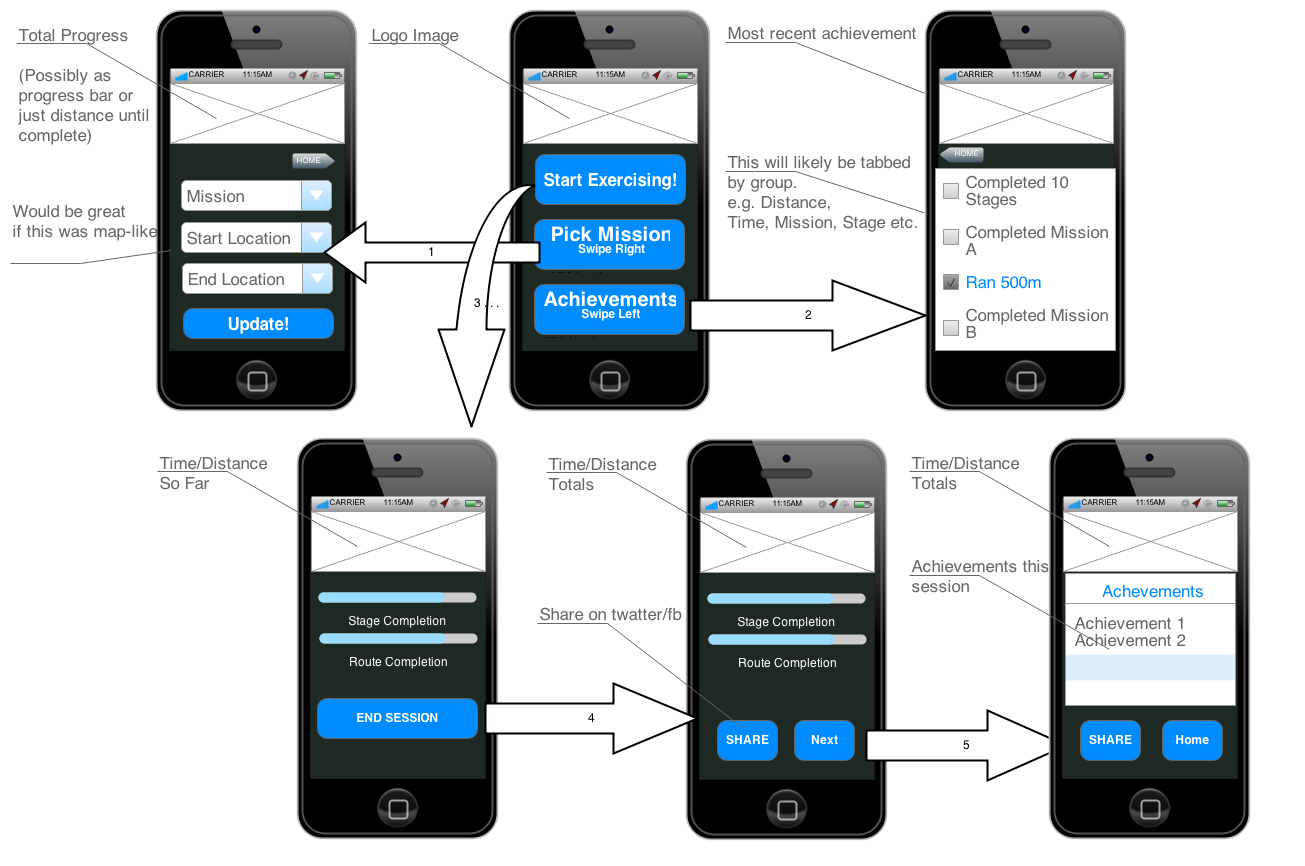
\includegraphics[width=\linewidth]{appendix/images/wireframes.png}
  \caption{Inital sketch of wireframe ideas}
  \label{wireframes_2}
\end{figure}

\chapter{Installation Instructions}
\label{ch:install_appendix}
The code can be checked out using git by executing the following command in the terminal:

\noindent See the following command :
\begin{lstlisting}[language=bash]
  $ git clone git@github.com:marinamarina/sure-thing.git
\end{lstlisting}

Installation instructions are found at the following url:

\url{https://www.github.com:marinamarina/sure-thing/blob/master/README.md}.


If any issues arise regarding installation of any part of the system, do not hesitate to contact me at 1014481@rgu.ac.uk

\chapter{Credits}
\label{ch:credits_appendix}
Some the application's code was taken from the GitHub repository accompanying the book by Miguel Grindberg "Flask Web Development" \citep{book:Grindberg2014FlaskWebDevelopment}. Below are listed the components of the system that rely on this code to some extent:

\begin{itemize}
	\item user authentication, account verification
	\item basic test suite
	\item user authentication test suite
\end{itemize}

Some of the handy decorator functions used in the Python code were taken from Flask documentation \citep{documentation:Flask,}, section "View Decorators".

\chapter{Project Management}
\label{ch:pm_appendix}
As it can already become apparent, the project was not developed following a single software development methodology. Different techniques from various methodologies were used for the project duration. For example, some of the planning was made beforehands in the traditional, Waterfall approach fashion, for example researching the project background, defining application requirements, sketching the application wireframes, etc. On the other hand, some of the design techniques were adopted from the Agile methodology, namely user stories and scenarios. 

The project implementation phase was carried out in the iterative manner. At the stage of defining the project requirements, the application functionality was divided into clearly defined units (so called "high-level features" introduced in the chapter "Requirements Analysis" \ref{ch:requirementanalysis}), each associated with an implementation iteration. Excel sheets were used for defining the set of tasks for each iteration. GitHub issue tracker was also used as a supporting productivity tool for this project. Code related tasks were recorded as "issues" for the project GitHub repository. In general, the GitHub issue tracker appeared to be a very efficient tool for keeping the focus. 

\chapter{Another Appendix}

This appendix makes use of the \emph{rotating} package to rotate both figures and tables ninety degrees allowing for large datasets and illustrations to be represented.

\begin{sidewaystable}
\begin{center}
   \begin{tabular}{llllllllll} 
   \toprule
   \textbf{Heading 1} & \textbf{Heading 2}  & \textbf{Heading 3}  & \textbf{Heading 4}  & \textbf{Heading 5}  & \textbf{Heading 6}  & \textbf{Heading 7}  & \textbf{Heading 8}  & \textbf{Heading 9}  & \textbf{Heading 10}  \cr
   \midrule
   aaa & bbbb & cccc & dddd & eeee & ffff & gggg & hhhh & iiii & jjjj \cr 
   aaa & bbbb & cccc & dddd & eeee & ffff & gggg & hhhh & iiii & jjjj \cr 
   aaa & bbbb & cccc & dddd & eeee & ffff & gggg & hhhh & iiii & jjjj \cr 
   aaa & bbbb & cccc & dddd & eeee & ffff & gggg & hhhh & iiii & jjjj \cr 
   aaa & bbbb & cccc & dddd & eeee & ffff & gggg & hhhh & iiii & jjjj \cr 
   aaa & bbbb & cccc & dddd & eeee & ffff & gggg & hhhh & iiii & jjjj \cr 
   \bottomrule
   \end{tabular}
\caption[A Short Caption for the table]{
	A much longer caption that will not be listed in the list of tables page.
}
\label{tab:sidewaysTable}
\end{center}
\end{sidewaystable}

\begin{sidewaysfigure}
\centerline{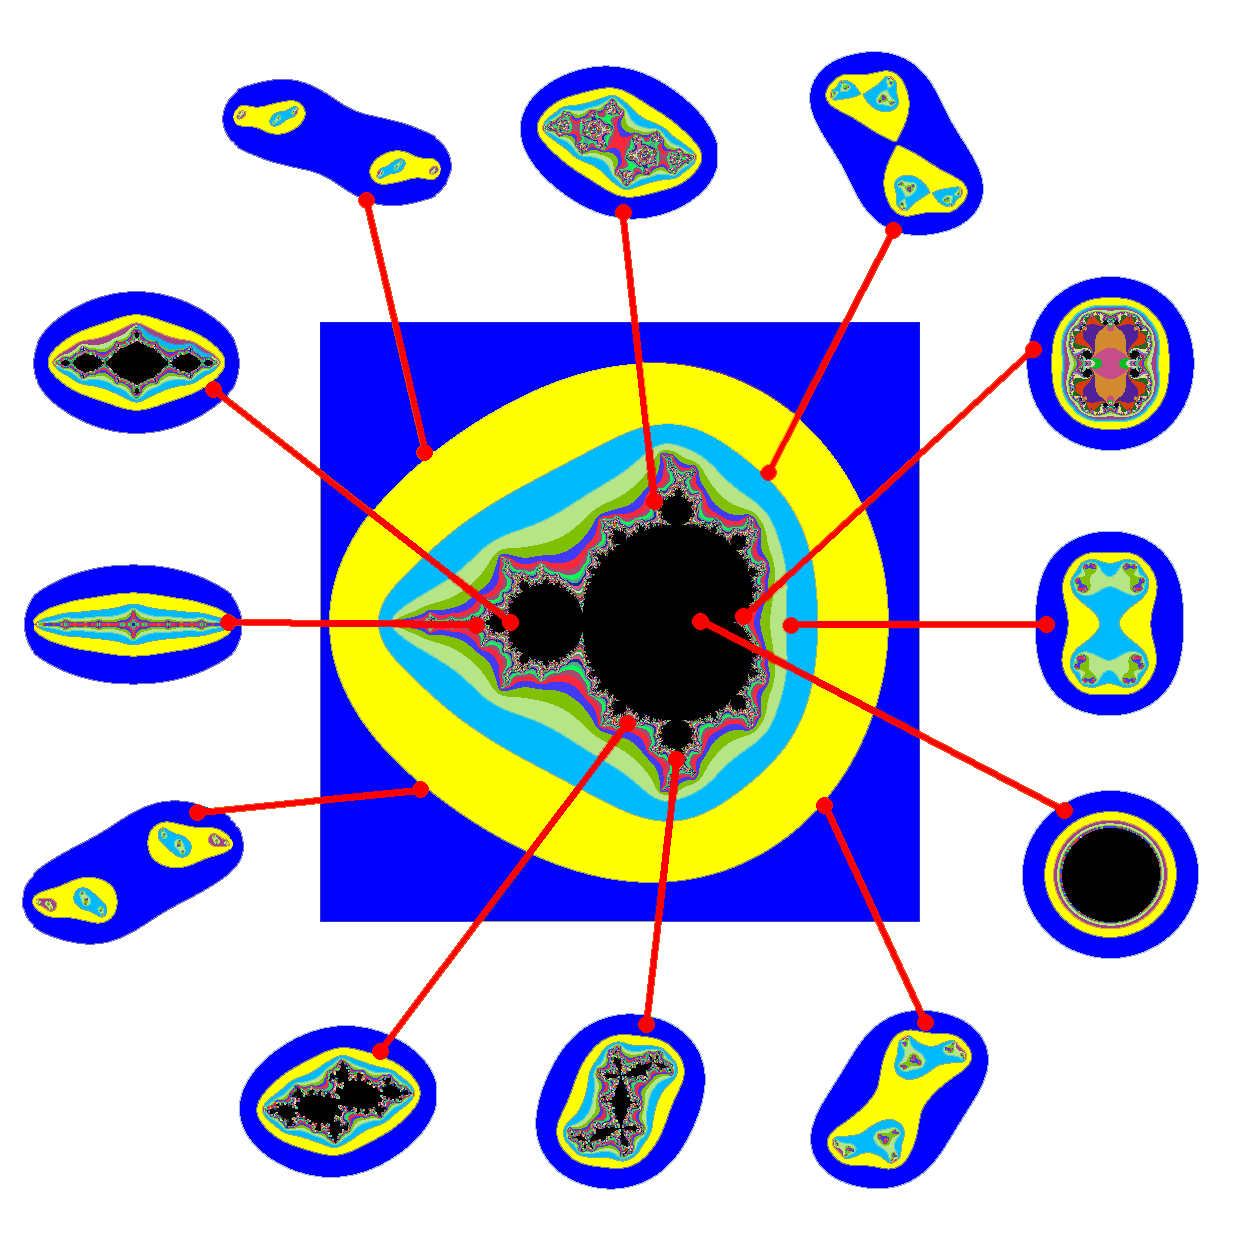
\includegraphics[width=0.8\textwidth,natwidth=610,natheight=642]{appendix/images/samplepng}}
\caption[A Sideways Figure]{
	A much longer caption that will not be listed in the list of figures page.
}
\label{fig:sidewaysFigure}
\end{sidewaysfigure}





\chapter{Presentation Slides}
\label{ch:slides_appendix}
The following is a weekly summary of the work carried during the development of this body of work. It covers tasks that were completed, tutorials that were worked through, articles that were read and reviews of discussions / meetings held with the project supervisor and other third parties. 




